\documentclass[tikz,border=8pt]{standalone}
\usepackage{amsmath}
\usepackage{pgfplots}
\pgfplotsset{compat=1.18}

\begin{document}
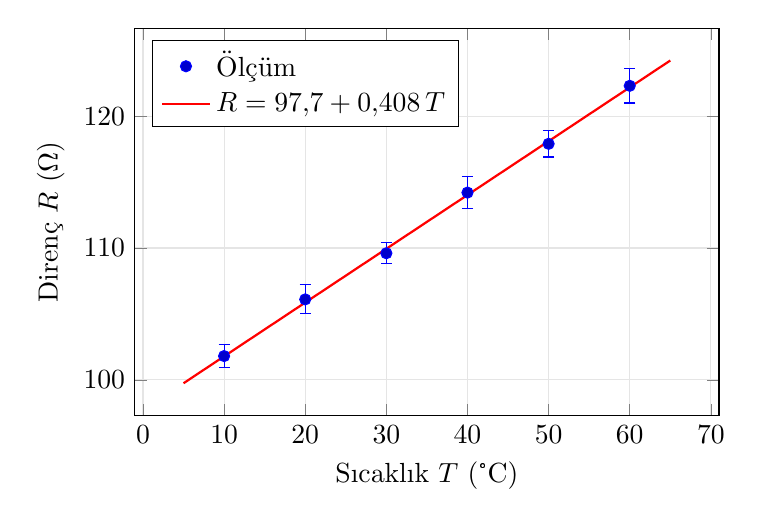
\begin{tikzpicture}
  \begin{axis}[
    width=9cm, height=6.5cm,
    xlabel={Sıcaklık $T$ (\textdegree C)},
    ylabel={Direnç $R$ ($\Omega$)},
    grid=major, grid style={gray!20},
    legend pos=north west, legend cell align=left,
  ]
    \addplot+[only marks, mark=*, error bars/.cd, y dir=both, y explicit]
      table[x=T, y=R, y error=dR, row sep=\\] {
        T  R     dR  \\
        10 101.8 0.9 \\
        20 106.1 1.1 \\
        30 109.6 0.8 \\
        40 114.2 1.2 \\
        50 117.9 1.0 \\
        60 122.3 1.3 \\
      };
    \addlegendentry{Ölçüm}
    \addplot[thick, red, domain=5:65] {97.7 + 0.408*x};
    \addlegendentry{$R = 97{,}7 + 0{,}408\,T$}
  \end{axis}
\end{tikzpicture}
\end{document}
